\documentclass[12pt, twoside]{article}
\usepackage[utf8]{inputenc}
\usepackage[english,russian]{babel}
\newcommand{\hdir}{.}

\usepackage{graphicx}
\usepackage{caption}
\usepackage{amssymb}
\usepackage{amsmath}
\usepackage{mathrsfs}
\usepackage{euscript}
\usepackage{upgreek}
\usepackage{array}
\usepackage{theorem}
\usepackage{graphicx}
\usepackage{subfig}
\usepackage{caption}
\usepackage{color}
\usepackage{url}

\DeclareMathOperator*{\argmin}{arg\,min}
\DeclareMathOperator*{\argmax}{arg\,max}

\usepackage[left=2cm,right=2cm,top=3cm,bottom=2cm,bindingoffset=0cm]{geometry}

\usepackage{fancyhdr}
\pagestyle{fancy}
\fancyhead{}
\fancyhead[LE,RO]{\thepage} 
\fancyhead[CO,CE]{Лекция 3}
\fancyhead[LO,LE]{Грабовой Андрей}

\begin{document} 

\begin{center}
{\LARGE\bf
Линейные модели и методы оптимиизации
}
\end{center}

\section{Регрессия}
$$\mathcal{D}^l = \{x_i, y_i\}_{i=1}^l, \quad x_i \in \mathbb{R},~y_i \in \mathbb{R}. \eqno(1.1)$$

Пусть имеется некоторая обучающая выборка $\mathcal{D}^l$ размера $l$ по которой мы хотим построить некоторую модель.

\paragraph{Определение 1.1:} Линейной моделью регрессии назовем функцию $\textbf{a}(x, \textbf{w})$  из (1.2), которая зависит от некоторого неизвестного параметра $\textbf{w} \in \mathbb{R}^n$.
$$\textbf{a}(x, \textbf{w}) = \sum_{j=1}^{n} w_j f_j(x), \eqno(1.2)$$
где $f_j(x)$ --- это функция которая по заданному объекту $x$ выдает $j$-й признак этого объекта.\\

Заметим, что вектор параметров $\textbf{w}$ является неизвестным и его нужно найти по заданной выборке $\mathcal{D}^l $

\paragraph{Определение 1.2:} Введем понятия функции потерь модели $\textbf{a}$ на некотором объекте $(x,y)\in \mathcal{D}^l$ следующиим образом:
$$\mathcal{L}(\textbf{w}, (x,y)) = (\textbf{a}(x, \textbf{w}) - y)^2. \eqno(1.3)$$

\paragraph{Определение 1.3:} Введем понятия функции потерь модели регрессии $\textbf{a}$ на выборке $\mathcal{D}^l$ следующим образом:
$$\mathcal{Q}(\textbf{w}) = \sum_{j=1}^{l} \mathcal{L}(\textbf{w}, (x_j,y_j)). \eqno(1.4)$$

Теперь, мы можем сформулировать задачу машинного обучения, как поиск $\textbf{w}$, такого что $\mathcal{Q}(\textbf{w})$ является минимальным. Формальная запись этого факта, это:

$$\hat{\textbf{w}} = \argmin_{\textbf{w}\in \mathbb{R}^n}\mathcal{Q}(\textbf{w}). \eqno(1.5)$$

Тогда после нахождения такого $\hat{\textbf{w}}$, мы получаем обученную линейную модель.

\section{Классификация}
$$\mathcal{D}^l = \{x_i, y_i\}_{i=1}^l, \quad x_i \in \mathbb{R},~y_i \in \{-1,+1\}. \eqno(2.1)$$

Пусть имеется некоторая обучающая выборка $\mathcal{D}^l$ размера $l$ по которой мы хотим построить некоторую модель.

\paragraph{Определение 2.1:} Линейной моделью классификации назовем функцию $\textbf{a}(x, \textbf{w})$  из (2.2), которая зависит от некоторого неизвестного параметра $\textbf{w} \in \mathbb{R}^n$.
$$\textbf{a}(x, \textbf{w}) = \text{sign}\sum_{j=1}^{n} w_j f_j(x), \eqno(2.2)$$
где $f_j(x)$ --- это функция которая по заданному объекту $x$ выдает $j$-й признак этого объекта.\\

\paragraph{Определение 2.2:} Введем понятия функции потерь модели классификации $\textbf{a}$ на некотором объекте $(x,y)\in \mathcal{D}^l$ следующиим образом:
$$\mathcal{L}(\textbf{w}, (x,y)) = -\textbf{a}(x, \textbf{w})\cdot y. \eqno(2.3)$$

\paragraph{Определение 2.3:} Введем понятия функции потерь модели регрессии $\textbf{a}$ на выборке $\mathcal{D}^l$ следующим образом:
$$\mathcal{Q}(\textbf{w}) = \sum_{j=1}^{l} \mathcal{L}(\textbf{w}, (x_j,y_j)). \eqno(2.4)$$

Теперь аналогично задачи регрессии сформулируем оптимизационную задачу:

$$\hat{\textbf{w}} = \argmin_{\textbf{w}\in \mathbb{R}^n}\mathcal{Q}(\textbf{w}). \eqno(2.5)$$

\section{Решение оптимизационной задачи}

\subsection{Производная}
$$f'(x) = \lim_{\Delta x \rightarrow 0}\frac{\Delta f}{\Delta x}. \eqno(3.1.1)$$

\begin{figure}[h!t]\center
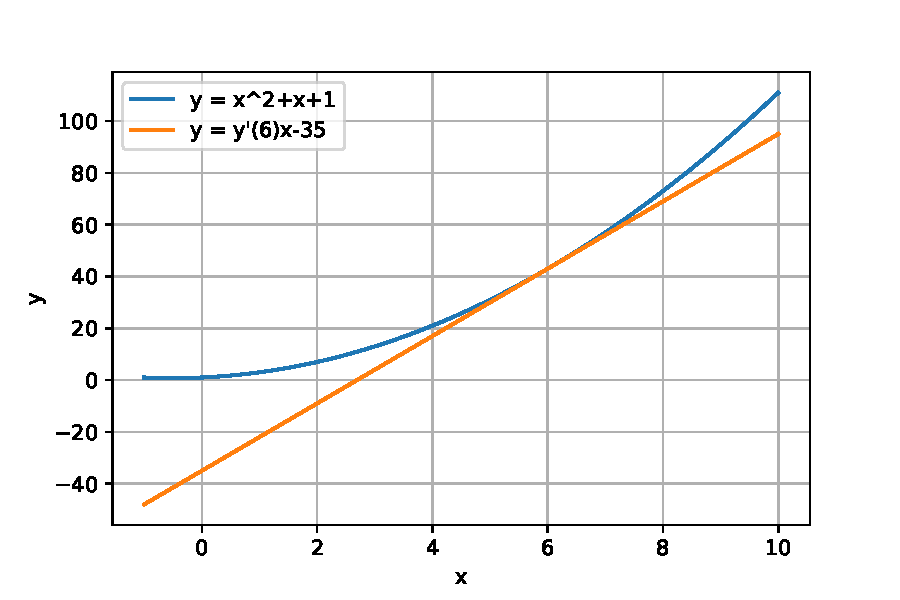
\includegraphics[width=0.7\textwidth]{Lecture_3_derivation.pdf}
\caption{График функции и касательная в точке$\textbf{a}$}
\label{Lecture_3_derivation}
\end{figure}

Будем использовать свойство знака производной. Знак производной указывает на то растет функция в этой точке или убывает, это свойство прямо следует из определения производной. Покажем этот факт:

 $$f'(x_0) =\lim_{\Delta x \rightarrow 0,~\Delta x>0}\frac{f(x_0+\Delta x) - f(x_0)}{\Delta x}, \eqno(3.1.2)$$
 
 Из уравнения (3.2) видно, что знак производной в точке $x_0$ равен знаку $f(x_0+\Delta x) - f(x_0)$, что  и требовалось показать.\\

Для примера из рис.~\ref{Lecture_3_derivation} $y'(6) = 13$. Тогда с этого следует, что функция в этой точке растет при увеличения $x$, тогда для того, чтобы найти минимальное значение $y$, нужно уменьшить $x$.\\

Вот мы пришли к выводу, что если у нас есть некоторая функция одного переменного, то для того, чтобы найти ее минимум нужно менять $x$ в противоположном направлении к знаку производной.

На этом базируется следующий итеративный подход к нахождению минимума функции.

\paragraph{Определение 3.1.1:} Итеративный процесс обозначает, что мы делаем что-то шаг за шагом.\\

Рассмотрим следующий итеративный процесс, для нахождения минимума одномерной функции $f(x)$ с областью определения $D_f$. 

1. Пусть имеется $x_0 \in D_f$ ---  некоторая точка из области определения функции.
2. Пересчитывать новую точку будем по формуле:
$$x_{n+1} = x_{n} - \alpha\cdot f'(x_{n}), \eqno(3.1.3)$$
где  $\alpha$ некоторое значение --- шаг который мы делаем, он может быть как и постоянным так и переменным. Мы будем пока считать его постоянным числом, например $0.0001$.

Мы научились находить минимум функции от скаляра. Но что же делать, для функции от вектора, которой является $\mathcal{Q}(\textbf{w})$.

\subsection{Градиент}
\paragraph{Определение 3.2.1:} Частной производной функции многих переменных $f(\textbf{x})$ по $x_j$ назовем производную функции $f'(x_j)$ считая все остальными переменные константой. Частная производная обозначается следующим образом:
$$\frac{\partial f}{\partial x_j} = f'_j(x_j), \eqno(3.2.1)$$
где $f'_j(x)$ --- это функция одной переменной, где все переменные кроме $j$-й фиксированы.

\paragraph{Определение 3.2.2:} Градиентом функции $f(\textbf{x})$ называется вектор $\nabla f(\textbf{x})$  элементы которого, это частные производные функции $f(\textbf{x})$.
$$\nabla f(\textbf{x}) = \begin{bmatrix}
\frac{\partial f}{x_1}\\
\frac{\partial f}{x_2}\\
\cdots\\
\frac{\partial f}{x_n}\\
\end{bmatrix}, \eqno(3.2.2)$$
где $x_1,~x_2,\cdots,~x_n$ --- компоненты вектора $\textbf{x}$.\\

По аналогии с функцией одного переменного можно определить итеративный процесс нахождения минимума функции многих переменных.

1. Пусть имеется $\textbf{x}^0 \in D_f$ ---  некоторая точка из области определения функции $f(\textbf{x})$.
2. Пересчитывать новую точку будем по формуле:
$$x^{n+1} = x^{n} - \alpha\cdot \nabla f(\textbf{x}^{n}), \eqno(3.2.3)$$
где  $\alpha$ некоторое значение --- шаг который мы делаем, он может быть как и постоянным так и переменным. Мы будем пока считать его постоянным числом, например $0.0001$.\\

Как видно все изменения в итеративной формуле это производная на градиент.

\subsection{Пример вычисления градиентов:}

$$f(x_1,x_2) = x_1^2 + x_2^2 \Rightarrow 
\nabla f(x_1, x_2) = \begin{bmatrix}
\frac{\partial f}{x_1}\\
\frac{\partial f}{x_2}\\
\end{bmatrix} = \begin{bmatrix}
2x_1\\
2x_2\\
\end{bmatrix}. \eqno(3.3.1)$$

$$f(x_1,x_2) = e^{x_1} + e^{x_2} + x_1x_2 \Rightarrow 
\nabla f(x_1, x_2) = \begin{bmatrix}
\frac{\partial f}{x_1}\\
\frac{\partial f}{x_2}\\
\end{bmatrix} = \begin{bmatrix}
e^{x_1}+x_2\\
e^{x_2}+x_1\\
\end{bmatrix}. \eqno(3.3.2)$$


\begin{thebibliography}{99}
	\bibitem{vokov}
	\textit{Воронцов К. В.} Машинное обучение // Годовой курс кафедры <<Интеллектуальные системы>> Москва, 2018.
	\url{http://www.machinelearning.ru/wiki/index.php?title=Vokov}
\end{thebibliography}

\end{document} 